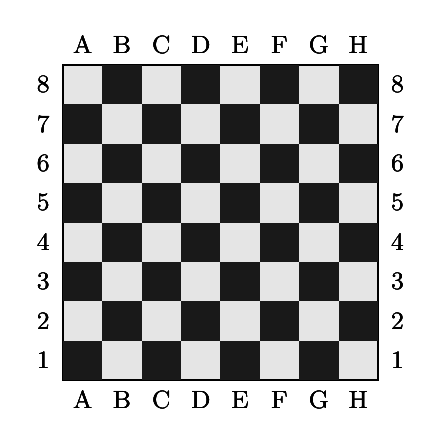
\begin{tikzpicture}[x=0.5cm,y=0.5cm]
	\draw[thick,fill=black!10] (0,0) rectangle (8,8);
	\foreach \x in {0,2,4,6} {
			\foreach \y in {0,2,...,6} {
					\fill[black!90] (\x,\y) rectangle +(1,1);
					\fill[black!90,shift={(1,1)}] (\x,\y) rectangle +(1,1);
				}
				\foreach[count=\x] \n in {A,...,H} {
					\node[shift={(-0.5,-0.5)}] at (\x,0) {\small \n};	
					\node[shift={(-0.5,8.5)}] at (\x,0) {\small \n};	
					\node[shift={(-0.5,-0.5)}] at (0,\x) {\small \x};
					\node[shift={(8.5,-0.5)}] at (0,\x) {\small \x};
				}
		}
\end{tikzpicture}
